% =============================================================================
% Paper v2 — assembled shell. Every metric reaches this document through
% numbers_v2.tex, which is regenerated from the run artifacts by
% 02_code/06_emit_macros_v2.py. Reported metrics use generated macros.
%
% Build without statistical recomputation: see
% WORKDIR/sdd/2026-09-09-no-recompute-closure/build_without_recompute.py.
% Verify reported numbers: python 02_code/08_check_numbers_v2.py.
% =============================================================================
\documentclass[twocolumn, 10pt]{article}

\makeatletter
\providecommand{\kscntformat}[3]{}
\providecommand{\@titleKor}{}
\providecommand{\@authorKor}{}
\makeatother

\usepackage{icicpe}
\renewenvironment{keyword}{%
 \list{}{\setlength{\leftmargin}{0.8cm}}%
 \small\item\relax\textbf{Keywords: }}%
 {\vspace{0.7cm}}
\usepackage[utf8]{inputenc}
\usepackage[pdfencoding=auto]{hyperref}
\usepackage{url}
\usepackage{amsmath}
\usepackage{amssymb}
\usepackage{bm}
\usepackage{graphicx}
\usepackage{booktabs}
\usepackage[symbol]{footmisc}
\usepackage{balance}

\graphicspath{{figures/}}

% --- auto-generated numbers: the single source of truth -----------------
% AUTO-GENERATED by emit_macros_v2.py - do not edit by hand
\newcommand{\vCorpus}{112{,}467}
\newcommand{\vTrain}{89{,}973}
\newcommand{\vVal}{11{,}247}
\newcommand{\vTest}{11{,}247}
\newcommand{\vDupsBc}{858}
\newcommand{\vDupsFeat}{3{,}372}
\newcommand{\vPosRate}{0.690}
\newcommand{\vSeed}{376}
\newcommand{\vNFeat}{67}
\newcommand{\vBLRFone}{0.890}
\newcommand{\vBLRLo}{0.886}
\newcommand{\vBLRHi}{0.894}
\newcommand{\vBLRPrec}{0.846}
\newcommand{\vBLRRec}{0.939}
\newcommand{\vBLRMcc}{0.610}
\newcommand{\vBLRFnr}{6.1\%}
\newcommand{\vBLRPrauc}{0.953}
\newcommand{\vBLRTrain}{6}
\newcommand{\vBRFFone}{0.945}
\newcommand{\vBRFLo}{0.942}
\newcommand{\vBRFHi}{0.949}
\newcommand{\vBRFPrec}{0.933}
\newcommand{\vBRFRec}{0.958}
\newcommand{\vBRFMcc}{0.819}
\newcommand{\vBRFFnr}{4.2\%}
\newcommand{\vBRFPrauc}{0.989}
\newcommand{\vBRFTrain}{132}
\newcommand{\vBXGBFone}{0.949}
\newcommand{\vBXGBLo}{0.946}
\newcommand{\vBXGBHi}{0.953}
\newcommand{\vBXGBPrec}{0.936}
\newcommand{\vBXGBRec}{0.963}
\newcommand{\vBXGBMcc}{0.832}
\newcommand{\vBXGBFnr}{3.7\%}
\newcommand{\vBXGBPrauc}{0.990}
\newcommand{\vBXGBTrain}{91}
\newcommand{\vBCatFone}{0.935}
\newcommand{\vBCatLo}{0.931}
\newcommand{\vBCatHi}{0.939}
\newcommand{\vBCatPrec}{0.932}
\newcommand{\vBCatRec}{0.938}
\newcommand{\vBCatMcc}{0.789}
\newcommand{\vBCatFnr}{6.2\%}
\newcommand{\vBCatPrauc}{0.985}
\newcommand{\vBCatTrain}{62}
\newcommand{\vDeltaFone}{+0.0041}
\newcommand{\vDeltaLo}{+0.0018}
\newcommand{\vDeltaHi}{+0.0063}
\newcommand{\vDeltaPgt}{$>$0.999}
\newcommand{\vDeltaB}{2{,}000}
\newcommand{\vSensDeltaFone}{+0.0016}
\newcommand{\vSensDeltaLo}{-0.0008}
\newcommand{\vSensDeltaHi}{+0.0041}
\newcommand{\vSensPgt}{0.905}
\newcommand{\vSensB}{2{,}000}
\newcommand{\vSensTableMatches}{3/4}
\newcommand{\vSensExactMatches}{1/4}
\newcommand{\vSensExactModel}{RF}
\newcommand{\vSensXgbThrRef}{0.435}
\newcommand{\vSensXgbThrRerun}{0.635}
\newcommand{\vSensXgbFoneRerun}{0.9469}
\newcommand{\vMlXgb}{0.7646}
\newcommand{\vMlRf}{0.6908}
\newcommand{\vMlLr}{0.4538}
\newcommand{\vDlBestName}{C2\_dmodel\_256}
\newcommand{\vDlBest}{0.6793}
\newcommand{\vDlWorst}{0.6215}
\newcommand{\vDlMean}{0.6506}
\newcommand{\vDlGap}{8.53}
\newcommand{\vDlWins}{8/8}
\newcommand{\vDlLosing}{10}
\newcommand{\vDlOf}{10}
\newcommand{\vDlNConfigs}{10}
\newcommand{\vDlArch}{depth, width, pure CNN, and pure Transformer}
\newcommand{\vDlCaveat}{}
\newcommand{\vReproChecks}{114}
\newcommand{\vDlTimeN}{4}
\newcommand{\vDlTimeOf}{10}
\newcommand{\vDlTimeLo}{1{,}271}
\newcommand{\vDlTimeHi}{6{,}697}
\newcommand{\vShapN}{2{,}000}
\newcommand{\vShapAgree}{3}
\newcommand{\vShapLead}{jumpi\_count}
\newcommand{\vShapDir}{positive}
\newcommand{\vShapGainLead}{external\_call\_count}
\newcommand{\vJacFive}{0.43}
\newcommand{\vJacFifteen}{0.25}
\newcommand{\vLeakVal}{555}
\newcommand{\vLeakRate}{4.76\%}
\newcommand{\vLeakWorst}{double-spending}
\newcommand{\vLeakWorstRate}{32.7\%}
\newcommand{\vLeakWorstN}{17}
\newcommand{\vLeakWorstOf}{52}
\newcommand{\vLeakNextRate}{6.8\%}
\newcommand{\vCloneFam}{82}
\newcommand{\vCloneShare}{18.4\%}
\newcommand{\vRareAName}{double-spending}
\newcommand{\vRareAPrev}{0.35\%}
\newcommand{\vRareAXgb}{0.5000}
\newcommand{\vRareALeak}{32.7\%}
\newcommand{\vRareBName}{bad-randomness}
\newcommand{\vRareBPrev}{2.56\%}
\newcommand{\vRareBXgb}{0.6667}
\newcommand{\vRareBLeak}{1.8\%}
\newcommand{\vBestLabName}{unchecked-calls}
\newcommand{\vBestLabXgb}{0.9105}
\newcommand{\vFlagRate}{71\%}
\newcommand{\vWorkloadRed}{1.4}
\newcommand{\vRunGpu}{Tesla T4}
\newcommand{\vRunDlBestTest}{0.6539}
\newcommand{\vHexVocab}{1{,}405}
\newcommand{\vHexNamed}{16}


\title[english]{Lightweight Machine Learning for Smart-Contract
Vulnerability Detection from EVM Bytecode: Binary and Multi-Label
Classification with a Deep-Learning Comparator}

\author[english]{
Sergei Solovev\\
\texttt{sssolovjov@gmail.com}
}

\finalcopy

\begin{document}
\raggedbottom

\twocolumn[
\maketitle
\begin{abstract}
Most Ethereum mainnet contracts are deployed without verified
source~\cite{cobra,scannerstudy}, which places them beyond source-level
analysers such as Slither. We study whether a lightweight classifier over
\vNFeat{} features extracted from EVM bytecode can predict Slither's findings,
as a prioritisation aid where source is absent. On \vCorpus{} Slither-labelled
contracts, duplicates are removed on the feature vector the models actually
see, hyperparameters are tuned on training folds, thresholds are chosen on
validation, and the test split is read once. Gradient boosting detects
any-vulnerability contracts at $F_1 =$ \vBXGBFone{} {[}\vBXGBLo, \vBXGBHi{]}
with a false-negative rate of \vBXGBFnr; its paired advantage over a random
forest is small and environment-sensitive, since a controlled rerun's
interval crosses zero. On the eight-class task, XGBoost (macro-$F_1$
\vMlXgb) scores higher than every one of \vDlNConfigs{} Conv-Transformer
configurations (best \vDlBest). A provenance audit found that the
comparator's token sequences were produced by disassembling hexadecimal text
without decoding it to bytes, so that negative result holds for that
representation only, and the usual tabular-data explanation remains a
hypothesis. We also measure what the earlier, text-deduplicated split
leaked: \vLeakRate{} of its validation contracts had a feature-identical
twin in training, rising to \vLeakWorstRate{} for \vLeakWorst.
\end{abstract}

\begin{keyword}
smart contracts, EVM bytecode, vulnerability detection, feature engineering,
multi-label classification, tabular learning, data leakage, bootstrap
confidence intervals, DeFi security
\end{keyword}
]

\section{Introduction}\label{sec:intro-v2}

Decentralised finance holds tens of billions of dollars in total value
locked~\cite{defillama}, and public leaderboards record cumulative losses past USD~3~billion
from smart-contract exploits since 2016~\cite{rekt}. Many of the contracts holding
these assets are immutable after deployment, and while upgradeable proxy
patterns and operational controls such as pausing and monitoring exist,
pre-deployment and pre-interaction checks remain part of contract security.

Two distinct obstacles stand between a deployed contract and existing
analysis, and conflating them overstates the case. Source-level static
analysers such as Slither~\cite{slither} require Solidity source, which a
substantial fraction of mainnet-deployed contracts never publish---for those,
bytecode is the only universally available artefact. Symbolic executors such
as Mythril~\cite{mythril} and Manticore~\cite{manticore} do
\emph{not} share that limitation: both operate on EVM bytecode directly. Their
computational cost can grow with the number of execution paths. That
motivates studying screening methods, but this work does not measure a
matched cost advantage over those tools.

We study a candidate Tier-1 pre-filter: a bytecode predictor that could rank
contracts for further analysis. The evaluation concerns agreement with
analyser-derived labels, not the effectiveness of a deployed triage system.

\paragraph{Contributions.}
\textbf{(i)~A bytecode-only prediction baseline} over \vNFeat{} engineered
features mapped to the SWC registry~\cite{swcRegistry}, evaluated with a security-relevant metric suite (FNR, PR-AUC,
precision/recall at a validation-selected threshold).
\textbf{(ii)~A leakage-resistant evaluation protocol:} duplicates removed
in feature space, a three-way split with a build-time no-overlap invariant,
binary hyperparameter search confined to training folds, and
validation-selected thresholds before reference test evaluation.
\textbf{(iii)~A deep-learning comparator under the same protocol:}
\vDlNConfigs{} Conv-Transformer configurations, none of which scores higher
than gradient boosting on any class, on a token representation we later
found to be defective (Sec.~\ref{sec:methods}).

\paragraph{Relation to an earlier version of this work.}
An earlier preprint reported comparable headline numbers under a protocol we
now consider unsound: duplicates were removed on the raw bytecode string,
which left contracts that are bit-identical in feature space on both sides of
the split, and the search over hyperparameters was scored on the same data
used for reporting. The present numbers are produced under the protocol
described below (Sec.~\ref{sec:data-v2}), and we report both the corrected
results and the measured overlap. Because partition and protocol changed
together, the score differences do not isolate a causal effect of leakage.

% =============================================================================
% Paper v2 — results & methodology sections, written entirely against the
% auto-generated macros in numbers_v2.tex. No metric is ever typed by hand.
%
% This file is the answer to the v1 failure mode: numbers drifted between the
% prose, the figures, the README and the model card because each was edited
% independently. Here a number exists in exactly one place — the artifact —
% and reaches the page only through % AUTO-GENERATED by emit_macros_v2.py - do not edit by hand
\newcommand{\vCorpus}{112{,}467}
\newcommand{\vTrain}{89{,}973}
\newcommand{\vVal}{11{,}247}
\newcommand{\vTest}{11{,}247}
\newcommand{\vDupsBc}{858}
\newcommand{\vDupsFeat}{3{,}372}
\newcommand{\vPosRate}{0.690}
\newcommand{\vSeed}{376}
\newcommand{\vNFeat}{67}
\newcommand{\vBLRFone}{0.890}
\newcommand{\vBLRLo}{0.886}
\newcommand{\vBLRHi}{0.894}
\newcommand{\vBLRPrec}{0.846}
\newcommand{\vBLRRec}{0.939}
\newcommand{\vBLRMcc}{0.610}
\newcommand{\vBLRFnr}{6.1\%}
\newcommand{\vBLRPrauc}{0.953}
\newcommand{\vBLRTrain}{6}
\newcommand{\vBRFFone}{0.945}
\newcommand{\vBRFLo}{0.942}
\newcommand{\vBRFHi}{0.949}
\newcommand{\vBRFPrec}{0.933}
\newcommand{\vBRFRec}{0.958}
\newcommand{\vBRFMcc}{0.819}
\newcommand{\vBRFFnr}{4.2\%}
\newcommand{\vBRFPrauc}{0.989}
\newcommand{\vBRFTrain}{132}
\newcommand{\vBXGBFone}{0.949}
\newcommand{\vBXGBLo}{0.946}
\newcommand{\vBXGBHi}{0.953}
\newcommand{\vBXGBPrec}{0.936}
\newcommand{\vBXGBRec}{0.963}
\newcommand{\vBXGBMcc}{0.832}
\newcommand{\vBXGBFnr}{3.7\%}
\newcommand{\vBXGBPrauc}{0.990}
\newcommand{\vBXGBTrain}{91}
\newcommand{\vBCatFone}{0.935}
\newcommand{\vBCatLo}{0.931}
\newcommand{\vBCatHi}{0.939}
\newcommand{\vBCatPrec}{0.932}
\newcommand{\vBCatRec}{0.938}
\newcommand{\vBCatMcc}{0.789}
\newcommand{\vBCatFnr}{6.2\%}
\newcommand{\vBCatPrauc}{0.985}
\newcommand{\vBCatTrain}{62}
\newcommand{\vDeltaFone}{+0.0041}
\newcommand{\vDeltaLo}{+0.0018}
\newcommand{\vDeltaHi}{+0.0063}
\newcommand{\vDeltaPgt}{$>$0.999}
\newcommand{\vDeltaB}{2{,}000}
\newcommand{\vSensDeltaFone}{+0.0016}
\newcommand{\vSensDeltaLo}{-0.0008}
\newcommand{\vSensDeltaHi}{+0.0041}
\newcommand{\vSensPgt}{0.905}
\newcommand{\vSensB}{2{,}000}
\newcommand{\vSensTableMatches}{3/4}
\newcommand{\vSensExactMatches}{1/4}
\newcommand{\vSensExactModel}{RF}
\newcommand{\vSensXgbThrRef}{0.435}
\newcommand{\vSensXgbThrRerun}{0.635}
\newcommand{\vSensXgbFoneRerun}{0.9469}
\newcommand{\vMlXgb}{0.7646}
\newcommand{\vMlRf}{0.6908}
\newcommand{\vMlLr}{0.4538}
\newcommand{\vDlBestName}{C2\_dmodel\_256}
\newcommand{\vDlBest}{0.6793}
\newcommand{\vDlWorst}{0.6215}
\newcommand{\vDlMean}{0.6506}
\newcommand{\vDlGap}{8.53}
\newcommand{\vDlWins}{8/8}
\newcommand{\vDlLosing}{10}
\newcommand{\vDlOf}{10}
\newcommand{\vDlNConfigs}{10}
\newcommand{\vDlArch}{depth, width, pure CNN, and pure Transformer}
\newcommand{\vDlCaveat}{}
\newcommand{\vReproChecks}{114}
\newcommand{\vDlTimeN}{4}
\newcommand{\vDlTimeOf}{10}
\newcommand{\vDlTimeLo}{1{,}271}
\newcommand{\vDlTimeHi}{6{,}697}
\newcommand{\vShapN}{2{,}000}
\newcommand{\vShapAgree}{3}
\newcommand{\vShapLead}{jumpi\_count}
\newcommand{\vShapDir}{positive}
\newcommand{\vShapGainLead}{external\_call\_count}
\newcommand{\vJacFive}{0.43}
\newcommand{\vJacFifteen}{0.25}
\newcommand{\vLeakVal}{555}
\newcommand{\vLeakRate}{4.76\%}
\newcommand{\vLeakWorst}{double-spending}
\newcommand{\vLeakWorstRate}{32.7\%}
\newcommand{\vLeakWorstN}{17}
\newcommand{\vLeakWorstOf}{52}
\newcommand{\vLeakNextRate}{6.8\%}
\newcommand{\vCloneFam}{82}
\newcommand{\vCloneShare}{18.4\%}
\newcommand{\vRareAName}{double-spending}
\newcommand{\vRareAPrev}{0.35\%}
\newcommand{\vRareAXgb}{0.5000}
\newcommand{\vRareALeak}{32.7\%}
\newcommand{\vRareBName}{bad-randomness}
\newcommand{\vRareBPrev}{2.56\%}
\newcommand{\vRareBXgb}{0.6667}
\newcommand{\vRareBLeak}{1.8\%}
\newcommand{\vBestLabName}{unchecked-calls}
\newcommand{\vBestLabXgb}{0.9105}
\newcommand{\vFlagRate}{71\%}
\newcommand{\vWorkloadRed}{1.4}
\newcommand{\vRunGpu}{Tesla T4}
\newcommand{\vRunDlBestTest}{0.6539}
\newcommand{\vHexVocab}{1{,}405}
\newcommand{\vHexNamed}{16}
.
%
% Include from main_v2.tex AFTER % AUTO-GENERATED by emit_macros_v2.py - do not edit by hand
\newcommand{\vCorpus}{112{,}467}
\newcommand{\vTrain}{89{,}973}
\newcommand{\vVal}{11{,}247}
\newcommand{\vTest}{11{,}247}
\newcommand{\vDupsBc}{858}
\newcommand{\vDupsFeat}{3{,}372}
\newcommand{\vPosRate}{0.690}
\newcommand{\vSeed}{376}
\newcommand{\vNFeat}{67}
\newcommand{\vBLRFone}{0.890}
\newcommand{\vBLRLo}{0.886}
\newcommand{\vBLRHi}{0.894}
\newcommand{\vBLRPrec}{0.846}
\newcommand{\vBLRRec}{0.939}
\newcommand{\vBLRMcc}{0.610}
\newcommand{\vBLRFnr}{6.1\%}
\newcommand{\vBLRPrauc}{0.953}
\newcommand{\vBLRTrain}{6}
\newcommand{\vBRFFone}{0.945}
\newcommand{\vBRFLo}{0.942}
\newcommand{\vBRFHi}{0.949}
\newcommand{\vBRFPrec}{0.933}
\newcommand{\vBRFRec}{0.958}
\newcommand{\vBRFMcc}{0.819}
\newcommand{\vBRFFnr}{4.2\%}
\newcommand{\vBRFPrauc}{0.989}
\newcommand{\vBRFTrain}{132}
\newcommand{\vBXGBFone}{0.949}
\newcommand{\vBXGBLo}{0.946}
\newcommand{\vBXGBHi}{0.953}
\newcommand{\vBXGBPrec}{0.936}
\newcommand{\vBXGBRec}{0.963}
\newcommand{\vBXGBMcc}{0.832}
\newcommand{\vBXGBFnr}{3.7\%}
\newcommand{\vBXGBPrauc}{0.990}
\newcommand{\vBXGBTrain}{91}
\newcommand{\vBCatFone}{0.935}
\newcommand{\vBCatLo}{0.931}
\newcommand{\vBCatHi}{0.939}
\newcommand{\vBCatPrec}{0.932}
\newcommand{\vBCatRec}{0.938}
\newcommand{\vBCatMcc}{0.789}
\newcommand{\vBCatFnr}{6.2\%}
\newcommand{\vBCatPrauc}{0.985}
\newcommand{\vBCatTrain}{62}
\newcommand{\vDeltaFone}{+0.0041}
\newcommand{\vDeltaLo}{+0.0018}
\newcommand{\vDeltaHi}{+0.0063}
\newcommand{\vDeltaPgt}{$>$0.999}
\newcommand{\vDeltaB}{2{,}000}
\newcommand{\vSensDeltaFone}{+0.0016}
\newcommand{\vSensDeltaLo}{-0.0008}
\newcommand{\vSensDeltaHi}{+0.0041}
\newcommand{\vSensPgt}{0.905}
\newcommand{\vSensB}{2{,}000}
\newcommand{\vSensTableMatches}{3/4}
\newcommand{\vSensExactMatches}{1/4}
\newcommand{\vSensExactModel}{RF}
\newcommand{\vSensXgbThrRef}{0.435}
\newcommand{\vSensXgbThrRerun}{0.635}
\newcommand{\vSensXgbFoneRerun}{0.9469}
\newcommand{\vMlXgb}{0.7646}
\newcommand{\vMlRf}{0.6908}
\newcommand{\vMlLr}{0.4538}
\newcommand{\vDlBestName}{C2\_dmodel\_256}
\newcommand{\vDlBest}{0.6793}
\newcommand{\vDlWorst}{0.6215}
\newcommand{\vDlMean}{0.6506}
\newcommand{\vDlGap}{8.53}
\newcommand{\vDlWins}{8/8}
\newcommand{\vDlLosing}{10}
\newcommand{\vDlOf}{10}
\newcommand{\vDlNConfigs}{10}
\newcommand{\vDlArch}{depth, width, pure CNN, and pure Transformer}
\newcommand{\vDlCaveat}{}
\newcommand{\vReproChecks}{114}
\newcommand{\vDlTimeN}{4}
\newcommand{\vDlTimeOf}{10}
\newcommand{\vDlTimeLo}{1{,}271}
\newcommand{\vDlTimeHi}{6{,}697}
\newcommand{\vShapN}{2{,}000}
\newcommand{\vShapAgree}{3}
\newcommand{\vShapLead}{jumpi\_count}
\newcommand{\vShapDir}{positive}
\newcommand{\vShapGainLead}{external\_call\_count}
\newcommand{\vJacFive}{0.43}
\newcommand{\vJacFifteen}{0.25}
\newcommand{\vLeakVal}{555}
\newcommand{\vLeakRate}{4.76\%}
\newcommand{\vLeakWorst}{double-spending}
\newcommand{\vLeakWorstRate}{32.7\%}
\newcommand{\vLeakWorstN}{17}
\newcommand{\vLeakWorstOf}{52}
\newcommand{\vLeakNextRate}{6.8\%}
\newcommand{\vCloneFam}{82}
\newcommand{\vCloneShare}{18.4\%}
\newcommand{\vRareAName}{double-spending}
\newcommand{\vRareAPrev}{0.35\%}
\newcommand{\vRareAXgb}{0.5000}
\newcommand{\vRareALeak}{32.7\%}
\newcommand{\vRareBName}{bad-randomness}
\newcommand{\vRareBPrev}{2.56\%}
\newcommand{\vRareBXgb}{0.6667}
\newcommand{\vRareBLeak}{1.8\%}
\newcommand{\vBestLabName}{unchecked-calls}
\newcommand{\vBestLabXgb}{0.9105}
\newcommand{\vFlagRate}{71\%}
\newcommand{\vWorkloadRed}{1.4}
\newcommand{\vRunGpu}{Tesla T4}
\newcommand{\vRunDlBestTest}{0.6539}
\newcommand{\vHexVocab}{1{,}405}
\newcommand{\vHexNamed}{16}
.
% =============================================================================

\section{Related Work}\label{sec:relwork}

\paragraph{Bytecode-only detectors.}
A 2024 large-scale audit of 17 production
scanners~\cite{scannerstudy} on $\sim\!4$M Ethereum bytecodes reports
systematically poor coverage, motivating a fundamentally different
first stage. COBRA~\cite{cobra} introduces interaction-aware
bytecode embeddings and explicitly targets the unverified-contract
regime; ByteEye~\cite{byteeye} reports $+35\%$--$44\%$ $F_1$ for a
bytecode-GNN over prior bytecode baselines. SmartBugBert
\cite{smartbugbert} combines BERT and TF-IDF on opcode streams,
reaching $F_1\!\approx\!0.91$.

\paragraph{Multimodal and multi-agent LLMs.}
Agent4Vul~\cite{agent4vul} fuses a semantic and a bytecode-CFG
branch and reports $+3.6\%$--$16.3\%$ $F_1$, beating GPT-4o;
LLM-BSCVM~\cite{llmbscvm} reaches $F_1\!>\!0.91$ with multi-agent
auditors; SmartLLaMA~\cite{smartllama} reports $+10.4\%$ over prior
LLM baselines on ISSTA 2025; LLM-MAS~\cite{llmmas} surveys the
multi-agent design space. The 2025 ACM survey~\cite{learnSurvey}
catalogues 61 learning-based methods, noting that sub-$5\%$ gains on
$\le\!10^{3}$-contract benchmarks routinely lack confidence
intervals.

\paragraph{What this literature does not settle.}
Reported gains in this area are seldom accompanied by the two things
that would let a reader judge them: an interval around the estimate,
and a statement of how duplicates were removed before the split. We
supply both, and Sec.~\ref{sec:leak-v2} quantifies what the second
one is worth on this corpus. 

\section{Dataset and Protocol}\label{sec:data-v2}

\paragraph{Corpus and what a label means.}
We build on the Slither-audited smart-contract corpus of
Rossini~\cite{slitherAudited}, which pairs Etherscan-verified sources with
their deployed EVM bytecode and per-detector Slither reports. A contract is
positive for a class when the corpus records at least one Slither finding
whose detector maps to that class; the mapping from the 39~detector names to
the eight classes ships with our code
(\texttt{data/label\_mappings.json}), and detectors mapped to
\texttt{ignore} are dropped rather than silently folded into \emph{other}.

The mapping is by detector name alone. The released derivative carries only
the eight binary labels, so no severity or confidence filter is applied at
this stage and none can be recovered from it downstream. A positive therefore
means that Slither emitted a finding, not that the finding is reachable or
exploitable, and every metric in this paper should be read as agreement with
that emission. The eight classes are the corpus's own label set, only
partly aligned with the DASP taxonomy: access-control, arithmetic,
bad-randomness, reentrancy and unchecked-calls correspond to DASP categories,
\emph{locked-ether} is a Slither detector name, \emph{double-spending} is not
a DASP category, and DASP's denial-of-service, front-running and
time-manipulation categories have no label here. We keep the corpus's names
rather than renaming them to a taxonomy they do not match.

\paragraph{Slither labels as the operational target.}
Labels are produced by the Slither~\cite{slither} static analyser,
itself a widely adopted tool in real audit pipelines and the
de-facto Tier-2 consumer of our Tier-1 output. We therefore frame
agreement with Slither at scale not as a compromise, but as
\emph{the operational task by design}: a Tier-1 pre-filter whose
job is to prioritise which contracts a Slither / Mythril stack
should process first. Reported metrics are agreement with Slither
on bytecode the analyser could in principle inspect itself if
source were available; the value is delivered on the larger
fraction of mainnet where it is not. The 2024 large-scale scanner audit~\cite{scannerstudy}
reports that no production scanner reaches human-audit-level
recall at mainnet scale; achieving Slither-consistency at
${\sim}1$\,ms per contract is, in that landscape, an
operationally useful target whose validity is bounded by the
documented FPR/FNR of the upstream analyser.

\paragraph{Deduplication is the load-bearing preprocessing step.}
Solidity appends a CBOR metadata trailer to runtime bytecode, so two builds
of identical source differ only in their final bytes. Deduplicating on the
raw bytecode string — as is common, and as our own earlier pipeline did —
therefore lets near-identical contracts survive into both sides of a split.
Because our features are mnemonic-level counts, such contracts are
\emph{bit-identical in feature space}, and a tree ensemble can memorise them.
We remove duplicates twice. The first pass drops \vDupsBc{} contracts whose
stored instruction text is identical. Its implementation also attempts to cut
a CBOR trailer, but the field it operates on holds the converter's mnemonic
text rather than hexadecimal runtime bytecode
(Sec.~\ref{sec:methods}), so that cut is inert: re-applying it to the
released inputs leaves every sampled row unchanged. We therefore describe
this pass as exact-duplicate removal on instruction text, not as
metadata-aware normalisation. The second pass drops \vDupsFeat{} contracts
sharing a \vNFeat-dimensional feature vector, leaving \vCorpus{} contracts at
a positive rate of \vPosRate. The second pass is the one that bears the
weight: it operates on exactly what the models see, and
Sec.~\ref{sec:leak-v2} measures what its absence cost the earlier split.

\subsection{What the earlier split actually leaked}\label{sec:leak-v2}

Because the earlier split is published, the consequence can be measured, and the leak turns out not to be spread evenly over the task.

Of the validation contracts in that split, \vLeakVal{} (\vLeakRate) are
bit-identical in feature space to a training contract --- rows the model
could recognise rather than classify. Broken down by class, the exposure is
strikingly uneven. For \vLeakWorst{}, \vLeakWorstN{} of \vLeakWorstOf{}
validation positives (\vLeakWorstRate) have an exact twin in training; no
other class exceeds \vLeakNextRate. The cause is a single contract template:
\vCloneFam{} feature-identical deployments, which alone account for
\vCloneShare{} of that class in the training split. String-level
deduplication kept every copy, because each deployment carries its own
metadata trailer.

The prediction this makes is testable against the earlier paper's own
reported numbers, and it holds in both directions. On \vLeakWorst, the class
with \vLeakWorstRate{} exposure, the earlier version reported per-class
$F_1 = 0.6835$ where the corrected protocol yields \vRareAXgb{} --- a loss of
more than eighteen points. On \emph{bad-randomness}, exposed at
\vRareBLeak{} --- the low end of that range --- it reported $0.6302$ where we now
measure \vRareBXgb, a slight \emph{gain}. Two classes are not a statistical
argument, and we do not present them as one: they are the two for which the
earlier text published a per-class figure, and they sit at opposite ends of
the exposure range. 

This is also the answer to a defence the earlier version offered explicitly:
that because every model shared the same split, any leakage would inflate all
of them about equally and so leave model comparisons intact. Leakage concentrated in
one class does not shift the models equally --- it shifts them where that
class carries weight, which for a macro-averaged score over eight classes is
exactly where the rare classes sit.

\paragraph{Split.}
A stratified \vTrain/\vVal/\vTest{} train/validation/test split (seed
\vSeed) preserves the positive rate to three decimals in every fold. We
assert, as a build-time invariant, that no feature vector occurs in more
than one split; the assertion and the resulting SHA-256 digests of all three
files ship with the code. Hyperparameters and decision thresholds are
selected on validation only. \textbf{The test split is read exactly once,
for the numbers reported below.}

Reading the test split once has a cost: every number here comes
from one draw of the split. The bootstrap intervals quantify sampling
variability \emph{within} the \vTest{} test contracts, not variability across
alternative partitions of the corpus. We did not repeat the protocol under
other seeds, so the point estimates carry an unquantified split-to-split
component. The comparison the paper turns on is not delicate at that scale
--- \vDlGap~p.p.\ separating XGBoost from the strongest of \vDlNConfigs{}
deep configurations, with a per-class sweep in each.

\paragraph{Threats to validity.}
The split and deduplication procedure is stated in full so a reader can bound the residual risk.
\textbf{(a)~Duplicate removal:} performed twice before the split, on the
stored instruction text and on the \vNFeat-dimensional feature vector; the
no-overlap invariant is asserted at build time. Only the second pass is
load-bearing, for the reason given in Sec.~\ref{sec:data-v2}.
\textbf{(b)~Split methodology:} the stratified three-way split is
randomised at the contract level (\texttt{seed}=\vSeed) and preserves the
positive rate to three decimals in every fold.
\textbf{(c)~Compiler-metadata limitation:} we do not stratify by compiler
version, so bytecode produced by the same \texttt{solc} release may carry
correlated PUSH/PUSH4 patterns across folds. Feature-space deduplication
removes exact twins, not this weaker correlation.
\textbf{(d)~Residual family correlations:} address-grouped splitting was not
performed. Feature-space deduplication catches template deployments that are
\emph{identical} in the model's input, which is what
Sec.~\ref{sec:leak-v2} shows was the dominant effect here, but a template
family whose members differ in a handful of features survives it. Its size
is not measured here. We defer address-grouped re-splitting via the
Etherscan proxy-detection API, together with a temporal train/test cut, to
the extended version.

\begin{figure}[t]
\centering
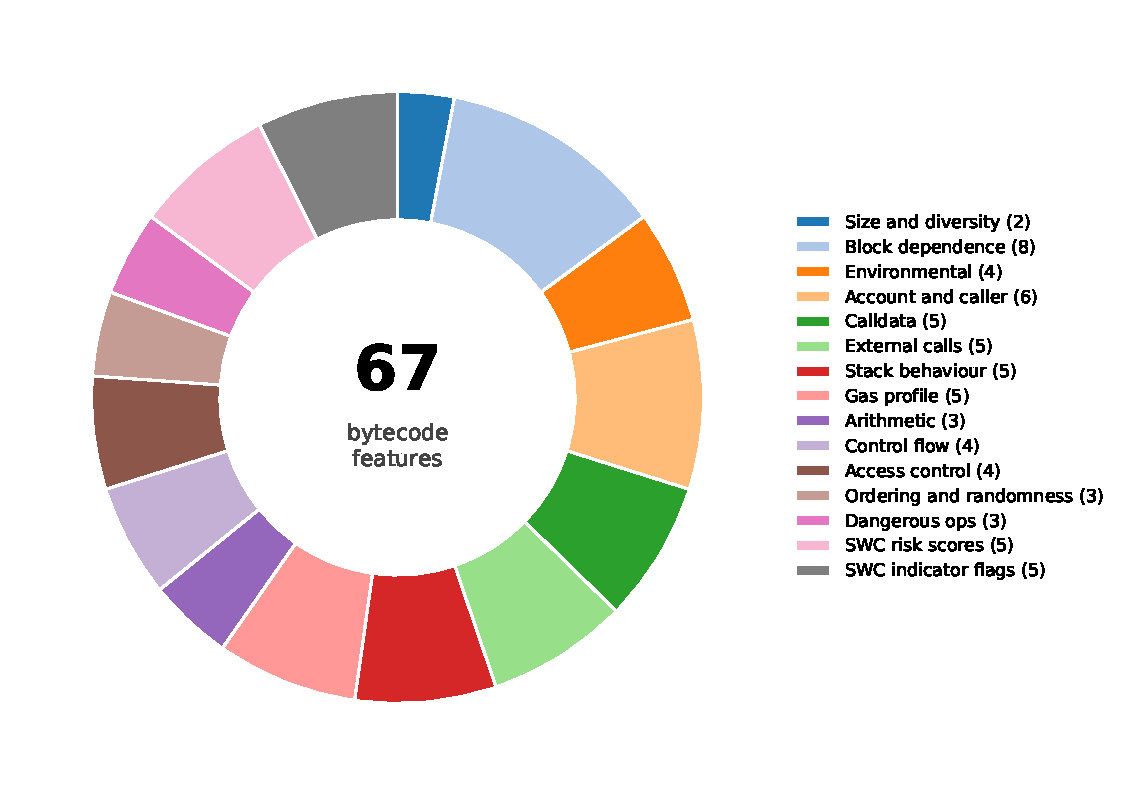
\includegraphics[width=0.95\columnwidth]{feature_categories_donut_v2.pdf}
\caption{The \vNFeat{} engineered bytecode features, grouped into fifteen
SWC-mapped semantic categories. Block-dependence is the largest group:
six opcode flags (\texttt{TIMESTAMP}, \texttt{NUMBER}, \texttt{DIFFICULTY},
\texttt{GASLIMIT}, \texttt{COINBASE}, \texttt{BLOCKHASH}) plus two
aggregates, reflecting how much of the SWC taxonomy turns on a contract
reading consensus state it cannot control. }
\label{fig:feat-cat}
\end{figure}

\section{Methods}\label{sec:methods}

\paragraph{Binary classification.}
Four models on the \vNFeat{} features: LogisticRegression
(\texttt{class\_weight=balanced}), RandomForest (200~trees), XGBoost tuned
with Optuna~\cite{optuna} (50~trials, 5-fold stratified CV \emph{inside the
training split}), and CatBoost~\cite{catboost} as an independent boosting
family that also exposes a different feature-importance measure
(PredictionValuesChange).

\paragraph{Multi-label classification.}
Three classical multi-label classifiers (LogReg, RandomForest, XGBoost)
wrapped in \texttt{sklearn.MultiOutputClassifier} predict the eight classes
of Sec.~\ref{sec:data-v2} (access-control, arithmetic, bad-randomness,
double-spending, locked-ether, other, reentrancy, unchecked-calls). Because
the split and \texttt{tree\_method=hist} are both deterministic, repeated
XGBoost seeds produce numerically identical predictions; seed variance is
therefore not an available uncertainty estimate, and we treat the eight
class-level $F_1$ values as the unit of paired inference instead. This is determinism, not replication: an identical model seed says nothing about the split seed (Sec.~\ref{sec:data-v2}).

\paragraph{Deep-learning comparator.}
A Conv-Transformer --- a depth-2 transformer over a 3-layer 1D-CNN
tokeniser, on 20{,}000-token sequences --- is trained on the same
multi-label split. The ablation covers loss (\texttt{BCE},
$+\!\texttt{pos\_weight}$, focal $\gamma\!=\!2$,
focal$\,+\,$\texttt{pos\_weight}, asymmetric~\cite{liu2021}, threshold
tuning) and architecture (\vDlArch).

\paragraph{Representation caveat.}
A provenance audit performed for the re-execution of
Sec.~\ref{sec:rerun-v2} found that the historical sequence converter passed
the hexadecimal \emph{string} to the disassembler without decoding it to
bytes. Every hexadecimal character was thus read as an opcode: the fitted
token vocabulary of \vHexVocab{} entries contains exactly \vHexNamed{} named
mnemonics, and they are precisely the opcodes whose values equal the ASCII
codes of the sixteen hexadecimal digits; on the synthetic input
\texttt{60016000} the historical path yields eight instructions where
decoding yields two \texttt{PUSH1}s. The \vNFeat{} numeric features are
unaffected, because their extractor decodes first. The comparator therefore
learned from an invertible but semantically scrambled encoding of the
bytecode, in which instruction boundaries and operands are not where a
sequence model would need them. Every deep-learning number in this paper is
a result for that legacy representation.

\paragraph{Bootstrap confidence intervals.}
Headline binary metrics carry stratified percentile bootstrap 95\% intervals
over the test split. Where two models are compared, the bootstrap is
\emph{paired} on the difference (Sec.~\ref{sec:binary-v2}): the models see the same contracts, so their errors are correlated.

\paragraph{Security-specific metrics.}
We report MCC~\cite{mcc} alongside $F_1$ because the corpus is \vPosRate{} positive: at that skew $F_1$ can be inflated by predicting the majority class generously, whereas MCC accounts for all four cells of the confusion matrix. We report the false-negative rate explicitly because in security a missed vulnerability is operationally costlier than a false alarm. Beyond
ranking we report PR-AUC, more informative than ROC-AUC for imbalanced
positives~\cite{prauc}, and we discuss \emph{Top-$k$ Recall} ($R@K$) --- the
fraction of vulnerabilities recovered when only the top $K\%$
most-suspicious contracts are forwarded downstream --- in
Sec.~\ref{sec:binary-v2}, where we show why it carries little information at
this positive rate.

\paragraph{Interpretability.}
Per-feature importance for both boosters side by side (XGBoost
gain~\cite{xgboost} versus CatBoost PVC~\cite{catboost}), plus SHAP
TreeExplainer~\cite{shap} attributions computed on validation samples ---
never on test, which under this protocol is read once. Where the two agree, the signal is more
likely to be in the data than in one model's fitting; Sec.~\ref{sec:ml-v2}
reports how far that agreement actually extends, which is less far than
the framing usually assumes.

\section{Binary Detection Results}\label{sec:binary-v2}

\begin{table*}[t]
\centering
\caption{Any-vulnerability detection on the held-out test split
(\vTest{} contracts). $F_1$ intervals are stratified percentile bootstrap,
$B\!=\!1000$. Thresholds were selected on the validation split; the test
split was read once. Training time is single-machine wall clock on identical
hardware, and is the basis for the compute comparison in
Sec.~\ref{sec:ml-v2}}
\label{tab:binary-v2}
\small
\begin{tabular}{lccccccc r}
\toprule
\textbf{Model} & $\bm{F_1}$ & \textbf{95\% CI} & \textbf{Prec.} &
\textbf{Rec.} & \textbf{FNR} & \textbf{MCC} & \textbf{PR-AUC} &
\textbf{Train (s)} \\
\midrule
XGBoost & \textbf{\vBXGBFone} & [\vBXGBLo, \vBXGBHi] &
 \vBXGBPrec & \vBXGBRec & \textbf{\vBXGBFnr} &
 \textbf{\vBXGBMcc} & \textbf{\vBXGBPrauc} & \vBXGBTrain \\
RandomForest & \vBRFFone & [\vBRFLo, \vBRFHi] &
 \vBRFPrec & \vBRFRec & \vBRFFnr &
 \vBRFMcc & \vBRFPrauc & \vBRFTrain \\
CatBoost & \vBCatFone & [\vBCatLo, \vBCatHi] &
 \vBCatPrec & \vBCatRec & \vBCatFnr &
 \vBCatMcc & \vBCatPrauc & \vBCatTrain \\
LogReg & \vBLRFone & [\vBLRLo, \vBLRHi] &
 \vBLRPrec & \vBLRRec & \vBLRFnr &
 \vBLRMcc & \vBLRPrauc & \vBLRTrain \\
\bottomrule
\end{tabular}
\end{table*}

XGBoost with Optuna-tuned hyperparameters reaches $F_1 =$ \vBXGBFone{}
[\vBXGBLo, \vBXGBHi] at a false-negative rate of \vBXGBFnr{}
(Table~\ref{tab:binary-v2}). Tuning used 50 trials optimising mean $F_1$
over a 5-fold stratified cross-validation \emph{inside the training split};
neither validation nor test participated in the search. 

\paragraph{Model comparison requires a paired test.}
Marginal confidence intervals for XGBoost and RandomForest overlap, and it
is tempting — but wrong — to conclude from that overlap that the models are
indistinguishable: the two are evaluated on the \emph{same} contracts, so
their errors are correlated and the marginal intervals are the wrong object.
The reference artifact records $\Delta F_1=\vDeltaFone$, 95\% CI
[\vDeltaLo, \vDeltaHi], $P(\Delta>0)$ \vDeltaPgt{}, over \vDeltaB{} resamples, but its fit-time environment
and fitted XGBoost model were not saved. The archived controlled rerun gives
\vSensDeltaFone{} [\vSensDeltaLo, \vSensDeltaHi],
$P(\Delta>0)=\vSensPgt$ (\vSensB{} resamples), so its interval crosses zero.
At table level \vSensTableMatches{} models match; only \vSensExactMatches{}
(\vSensExactModel) matches exactly, with all \vTest{} RF scores bit-identical.
For XGBoost the threshold moves \vSensXgbThrRef{}$\to$\vSensXgbThrRerun{}
and $F_1$ \vBXGBFone{}$\to$\vSensXgbFoneRerun. We retain the reference points,
treat the rerun as sensitivity analysis, and do not claim a statistically
resolved advantage across environments. The remaining mechanism is unknown;
versions, threads, platform and historical model state are hypotheses only.

\paragraph{Top-$k$ Recall has a ceiling here.}
A pre-filter is often judged by how many vulnerabilities it recovers inside
the top $K\%$ of its ranking. At a positive rate of $\pi_{+} = \vPosRate$
that metric is nearly uninformative: even a perfect ranker recovers at most
$K/\pi_{+}$ of the positives within the top $K\%$, giving ceilings of
\vCeilOne{} at $K\!=\!1$, \vCeilFive{} at $K\!=\!5$ and \vCeilTen{} at
$K\!=\!10$. Every model in Table~\ref{tab:binary-v2} sits at that ceiling,
so the metric separates nothing. We shift discrimination to PR-AUC, where the ordering is
\vBXGBPrauc{} (XGBoost) $>$ \vBRFPrauc{} (RandomForest) $>$ \vBCatPrauc{}
(CatBoost) $>$ \vBLRPrauc{} (LogReg) --- the same ordering as $F_1$. The
ceiling is a property of this corpus, not of the method: on a chain-wide
deployment stream, where the positive rate is far below \vPosRate,
Top-$k$~Recall regains its discriminating power and is the right metric to
report.

\paragraph{Throughput.}
Wall-clock cost per contract is dominated by feature extraction, not by
inference. On a 1{,}000-contract subsample, mean extraction time was
$0.97 \pm 0.21$~ms and tree-ensemble inference $0.04 \pm 0.01$~ms on a
single core of an Intel Xeon-class CPU (4~vCPU, 30~GB RAM), totalling
${\sim}1.0$~ms per contract. It was taken on the earlier extractor and has not been repeated under the present pipeline. The \vNFeat-dimensional vector adds two
derived counters computed from opcode tallies the disassembler has already
produced, which does not alter the cost structure --- disassembly dominates.

Extrapolating to ${\sim}10^{6}$~contracts/hour further \emph{assumes} linear
single-thread scaling and zero I/O cost. In production, parquet reads and
disassembler initialisation dominate at small batches, while parallelism is
trivial across cores and machines. The figure is an envelope, not a
guaranteed throughput.

\paragraph{Tier-1 operating envelope on this corpus, and where it does not
apply.}
A false-negative rate of \vBXGBFnr{} is a property of the
validation-selected threshold, and that threshold is permissive: at
precision \vBXGBPrec{} and recall \vBXGBRec{} on a corpus that is \vPosRate{}
positive, the filter forwards $\pi_{+}r/p \approx \vFlagRate$ of all
contracts. The workload reduction is therefore about
\vWorkloadRed$\times$, not two orders of magnitude, and on a corpus this
positive no threshold can do much better: the ceiling in the previous
paragraph is the same arithmetic seen from the other side. The two figures
are one fact, and quoting a small forwarding budget together with
\vBXGBFnr{} would state both halves of a contradiction.

The regime in which a Tier-1 filter pays for itself is the one this corpus
does not represent --- a deployment stream whose positive rate is far below
\vPosRate, where a fixed forwarding budget buys a materially different
recall. We have not measured such a stream, so we report the envelope as
measured here and treat the funnel argument as conditional on a base rate we
have not observed. What survives unconditionally is the per-contract cost
below, which is a property of the pipeline rather than of the corpus. 

\paragraph{Why not simply run Slither directly?}
A natural question, with three answers that survive the correction to our
protocol.
(i)~\textbf{No verified source.} Slither requires Solidity input, which a
substantial fraction of mainnet deployments never publish~\cite{cobra}; the
pipeline here is a layer over raw bytecode and applies universally.
(ii)~\textbf{Throughput gap.} Full Slither analysis runs
$\sim\!1$~s/contract end-to-end against $\sim\!1$~ms here --- three orders
of magnitude --- which is the difference between screening a deployment
stream and sampling it.
(iii)~\textbf{Streaming compatibility.} Classical inference is stateless and
embarrassingly parallel; a symbolic engine is neither.
The pipeline is therefore \emph{complementary} to Slither rather than a
replacement, and its labels come from Slither precisely because that is the
tool it feeds.

\section{Multi-Label Results and the Deep Comparator}\label{sec:ml-v2}

\begin{figure*}[t]
\centering

\includegraphics[width=\textwidth]{perlabel_f1_heatmap_v2.pdf}
\caption{Per-class $F_1$ on the held-out test split under the v2 protocol:
classical multi-label baselines (left of the first rule) against the
\vDlNConfigs{} Conv-Transformer configurations. Classes are ordered as in Sec.~\ref{sec:data-v2};
\textit{double-spending} is the rarest class and the one on which every model
degrades.}
\label{fig:heatmap-v2}
\end{figure*}

On the eight-class multi-label task, classical XGBoost reaches macro-$F_1 =$
\vMlXgb, RandomForest \vMlRf, and balanced logistic regression \vMlLr{} ---
the last collapsing on the rare classes and confirming that the regime is
not linearly separable.

\paragraph{Deep comparator.}
We train \vDlNConfigs{} Conv-Transformer configurations spanning loss
functions (BCE, positive-weighting, focal, asymmetric, threshold tuning) and
architectures (\vDlArch). Each is trained on
the same training split, early-stopped on an internal carve-out of that
split, and evaluated once on the same held-out test split as the classical
models. The best configuration, \vDlBestName, reaches macro-$F_1 =$
\vDlBest{} (worst \vDlWorst, mean \vDlMean), trailing XGBoost by
\vDlGap~p.p. Every one of these numbers is a result for the legacy token
representation described in Sec.~\ref{sec:methods}, in which the comparator
was fed the hexadecimal text of the bytecode rather than its decoded opcodes.
\vDlCaveat

\paragraph{Statistical framing.}
Per-class comparison over eight classes is a coarse instrument: with $n=8$
the smallest attainable two-sided $p$ from a sign test is $2/256 = 0.0078$,
so a clean sweep means ``eight out of eight'' and nothing stronger. The sign
test and the Wilcoxon signed-rank test applied to the same eight numbers are
the same evidence reported twice, not two independent confirmations; we
report the sign test only. XGBoost wins \vDlWins{} classes against
\vDlBestName{} at $p = \vDlPsign$ (Figure~\ref{fig:heatmap-v2}).

Across the family of \vDlNConfigs{} comparisons a Holm step-down correction admits nothing, and the reason is arithmetic: Holm requires the smallest
$p$ to fall below $\alpha/m = \vDlHolmThr$, while the sign test at $n=8$
cannot go below $2/256 = 0.0078$. Family-wise significance is therefore
unreachable \emph{by construction} at this design --- the binding constraint
is the number of classes, not the size of the effect. Holm's later thresholds do exceed $0.0078$, but step-down halts at the first non-rejection, so none of them is ever reached. What the data do support
is stated without inference: XGBoost wins every class against every deep
configuration. At the model level, \vDlLosing{} of
\vDlOf{} deep configurations fall below the classical baseline. We report
that count descriptively and attach no binomial $p$-value to it: the
configurations share one dataset and one feature representation, so the
independence assumption underlying such a test does not hold.

\paragraph{The hardest classes are bound by label scarcity, not capacity.}
Both the rarest classes are the hardest for every model in the comparison.
\vRareAName{} accounts for \vRareAPrev{} of test contracts and \vRareBName{}
for \vRareBPrev; classical XGBoost reaches \vRareAXgb{} and \vRareBXgb{} on
them, against \vBestLabXgb{} on the most common class,
\vBestLabName. The deep configurations degrade on the same rows and by more
(Figure~\ref{fig:heatmap-v2}), which is the opposite of what extra capacity
would buy if capacity were the constraint. Under class imbalance this severe
the deep model has \emph{less} headroom, not more.

We draw an explicit line here. Sec.~\ref{sec:leak-v2} showed that
\vLeakWorst{} was also the class most inflated by the earlier protocol, so
its low score under the corrected protocol has two contributions that this
design cannot separate: genuine difficulty, and the removal of contracts the
earlier model could recognise. What can be said is that the difficulty is
real --- the class is rare in a corrected corpus too --- and that its
earlier score was not.

\paragraph{Compute cost.}
The classical models train on a single CPU core in the times listed in
Table~\ref{tab:binary-v2}; the binary XGBoost fit, including its Optuna
search, takes \vBXGBTrain{}~s. The deep configurations train on a GPU; wall-clock training time survives for \vDlTimeN{} of the
\vDlTimeOf{} configurations, ranging from \vDlTimeLo{} to \vDlTimeHi{}~s.
The training time of the classical multi-label baseline --- the model that
actually wins the comparison --- was not recorded at all.

Three gaps therefore separate these timings from a compute comparison: the
classical side of the multi-label task is untimed, the classical figures that
do exist come from the binary task, and CPU seconds and GPU seconds are not
the same unit. We give the measurements and draw no ratio from them. The
earlier version did draw one, a $30\times$ ratio from a mean over the runs
that happened to carry a timestamp, read as a mean over all \vDlTimeOf. The
surviving timings therefore neither compare compute budgets nor establish
that any configuration was trained sufficiently.

\paragraph{Interpretability.}
Attributions come from a protocol-matched refit using the recorded XGBoost
hyperparameters on \vShapN{} validation samples; the unsaved historical fit
behind Table~\ref{tab:binary-v2} is not being explained. We use split gain,
which counts where the trees found their cuts, and mean absolute
SHAP, which counts how much each feature moves the output.

They share a core and diverge beyond it. \vShapAgree{} of
the top five appear in both lists --- \texttt{external\_call\_count}, \texttt{call\_gas\_limit\_ops} and \texttt{jumpi\_count} --- but the
agreement does not survive lengthening them: the Jaccard overlap
falls from \vJacFive{} at $K=5$ to \vJacFifteen{} at $K=15$.
Two rankings of one fit agreeing on part of their heads is weaker
evidence than a single ordering would suggest, and we report it as
such.

Direction is the more useful signal. Every feature in the SHAP top five except \texttt{conditional\_branching\_ratio} pushes the classifier toward ``vulnerable'' as its value rises,
which is the sign an auditor would predict for external calls and
branching complexity. We note one departure from the earlier
version, which built its account on \texttt{has\_external\_calls}: that
feature leads neither ranking here, while \vShapLead{}
leads the SHAP one. The earlier ranking came from the leaking split,
so the overlap that does exist is worth stating and not worth
leaning on.



\section{End-to-End Re-Execution}\label{sec:rerun-v2}

The numbers above come from a pipeline of numbered scripts whose fitted
models and fit-time environment were not saved (Sec.~\ref{sec:binary-v2}). To
close that gap from the other side, the author's original experiment notebook
was run to completion on a Kaggle \vRunGpu: it trains \vRunStages{} model
stages, seven classical and \vRunDl{} deep, ranks them on validation,
freezes the multi-label logistic reference, the validation-selected deep
configuration and the binary logistic reference before any test access, and
then reads the test split once. The notebook, its artifacts and a script that
recomputes every number below are released with this version, where the run's
operational detail is documented.

\begin{table}[t]
\centering
\caption{Reference pipeline against the end-to-end re-execution. The
re-execution scored only its frozen final set on the test split, so the lower
block compares its validation scores with the reference test scores and the
two columns are not like for like. The strongest deep configuration is
\vDlBestName{} in the reference and the re-execution selects the same one.
Binary LogReg reproduces to three decimals; multi-label LogReg differs
because the notebook standardises inputs for that reference and the script
did not.}
\label{tab:rerun-v2}
\footnotesize
\setlength{\tabcolsep}{4pt}
\begin{tabular}{@{}lcc@{}}
\toprule
 & \textbf{Reference} & \textbf{Re-exec.} \\
\midrule
\multicolumn{3}{@{}l}{\emph{Test split, both}} \\
Binary LogReg $F_1$ & \vBLRFone & \vRunBLRFone \\
Binary LogReg MCC & \vBLRMcc & \vRunBLRMcc \\
Binary LogReg PR-AUC & \vBLRPrauc & \vRunBLRPrauc \\
Multi-label LogReg macro-$F_1$ & \vMlLr & \vRunMlLr \\
Best deep config., macro-$F_1$ & \vDlBest & \vRunDlBestTest \\
\midrule
\multicolumn{3}{@{}l}{\emph{Reference (test) vs.\ re-exec.\ (validation)}} \\
Best deep config., macro-$F_1$ & \vDlBest & \vRunDlBestVal \\
XGBoost macro-$F_1$ & \vMlXgb & \vRunMlXgbVal \\
XGBoost $-$ best deep (p.p.) & \vDlGap & \vRunGapVal \\
Binary XGBoost PR-AUC & \vBXGBPrauc & \vRunBXGBPraucVal \\
Binary XGBoost MCC & \vBXGBMcc & \vRunBXGBMccVal \\
\bottomrule
\end{tabular}
\end{table}

\paragraph{What agrees.}
The binary logistic reference reproduces to three decimals
(Table~\ref{tab:rerun-v2}): the same standardised inputs, the same
deterministic solver and the same released split give the same $F_1$, MCC and
PR-AUC. The re-execution independently selects \vRunDlBestName{} as the
strongest deep configuration, now on validation (\vRunDlBestVal), and
XGBoost again beats every deep configuration, by \vRunGapVal~p.p.\ on
validation against \vDlGap~p.p.\ on the reference test split. Both pipelines
consume the same legacy token representation
(Sec.~\ref{sec:methods}), so this agreement establishes that the ordering is
not an artefact of the original scripts. It is not independent evidence about
deep learning on correctly decoded opcodes, and we do not read it as such.

\paragraph{What differs, and why.}
The multi-label logistic reference rises from \vMlLr{} to \vRunMlLr{} because
the notebook standardises its inputs and the historical script did not; that
difference measures standardisation, not reproduction. The selected deep
configuration reaches \vRunDlBestTest{} on the test split against \vDlBest{}
in the reference, under last-epoch rather than best-epoch weights, a resumed
training chain, and a single seed in both runs; we do not apportion the gap
among the three. Separately, tuning the four loss-variant thresholds on the
same validation split that selected them moves their macro-$F_1$ by
\vRunBFiveLo{} to \vRunBFiveHi. That is a threshold-sensitivity
diagnostic, computed after the freeze and outside model selection, on the
split that chose the thresholds; it estimates nothing about generalisation.

\paragraph{What the re-execution does not establish.}
It reads the same test split that Sec.~\ref{sec:ml-v2} read. Two reads of one
partition by two pipelines are still one partition, and any later change
motivated by either result cannot be confirmed on it. The
corrected-representation experiment that Sec.~\ref{sec:methods} calls for is
specified in the archive and has not been run (Sec.~\ref{sec:disc}).

\section{Discussion and Future Work}\label{sec:disc}

\paragraph{What the comparator's result does and does not show.}
The \vNFeat{} engineered features --- opcode counts, control-flow
statistics, gas aggregates, SWC-aligned risk scores --- form a
mid-dimensional tabular representation, the regime in which tree-based
ensembles are reported to outperform deep networks~\cite{grinsztajn2022,
shwartz2022}. That is one candidate explanation for the gap measured here,
and it is not established. The comparator saw a hexadecimal-character
encoding of the bytecode (Sec.~\ref{sec:methods}): invertible, so no
information was destroyed, but with every instruction boundary and every
\texttt{PUSH} operand displaced, and a network that must first learn to pair
hexadecimal digits into bytes is handicapped for a reason unrelated to the
tabular regime. This design cannot separate the two explanations, so the
cause of the gap remains a hypothesis. What is measured is narrower: on this
corpus, under this protocol, with this representation, gradient boosting on
\vNFeat{} features scores higher on every class.

\paragraph{Future work.}
The natural way out of the tabular regime is to carry structure end to end: a
bytecode-CFG GNN branch (COBRA~\cite{cobra}, ByteEye~\cite{byteeye}), a
multimodal model fusing source and CFG (Agent4Vul~\cite{agent4vul},
LLM-BSCVM~\cite{llmbscvm}, SmartLLaMA~\cite{smartllama}), or a multi-agent
auditor stack (LLM-MAS~\cite{llmmas}). These target the source-available
portion of mainnet at orders of magnitude more compute and are complementary
to a cheap Tier-1 filter rather than competing with it. A companion
preprint~\cite{preprintRAG} documents a sign reversal in a small-sample RAG
ablation, which is what first pushed us toward interval reporting; the 2025
ACM survey~\cite{learnSurvey} confirms that sub-$5\%$ gains on
$\le\!10^{3}$-contract benchmarks routinely arrive without them.
The nearest step is not a larger model but a corrected input: decode the
bytecode before disassembly, re-split the corpus by contract family, and
confirm on a partition that excludes every contract of the present test
split. That protocol is written and released with the archive; its execution
is future work.

\paragraph{Limitations.}
\textbf{(i)~The label ceiling.} Reported metrics are bounded by Slither's own
label quality on the corpus where Slither was applied. The model can at best
approximate Slither's recall on bytecode that Slither could itself have
processed given source. The operationally useful value-add is therefore
confined to two regimes: coverage extension to the mainnet fraction without
verified source, where the alternative signal is the empty set; and
constant-time triage when prioritising large unverified batches. Detecting
vulnerabilities beyond Slither's own capability --- including the residual
false negatives documented by the 2024 scanner audit~\cite{scannerstudy} ---
requires labels from mutation benchmarks (SolidiFI~\cite{solidifi}) or
human-curated corpora, retraining under matched label semantics, and a
domain-shift analysis we treat as separate work.
\textbf{(ii)~One split and incomplete fit provenance.} The bootstrap covers
sampling within one test split, not alternative partitions. Reference
artifacts preserve scores but not fitted models or fit-time environment; the
rerun matches \vSensTableMatches{} models at table level and
\vSensExactMatches{} exactly, moving the paired interval across zero.
\textbf{(iii)~Resolution of the paired tests.} With eight classes, a sign
test cannot produce a two-sided $p$ below $0.0078$, so family-wise
significance across \vDlNConfigs{} comparisons is unreachable by
construction. We report the sweep descriptively and let the effect size carry
the argument.
\textbf{(iv)~Attribution agreement is modest.} Split gain and mean
absolute SHAP, computed on the same protocol-matched refit, share three of their top five
features and less beyond that. We report the overlap rather than treat it
as corroboration.
\textbf{(v)~Legacy sequence representation.} The deep comparator's inputs
were produced by disassembling hexadecimal text without decoding it
(Sec.~\ref{sec:methods}); its results characterise that representation, not
canonical EVM opcode sequences. The numeric features are unaffected.
\textbf{(vi)~Re-execution scope.} The end-to-end run of
Sec.~\ref{sec:rerun-v2} is a resumed, single-seed execution that scored only
its frozen three models on the test split and retained last-epoch weights;
it reproduces the ordering and the binary logistic reference, not every
number.


\section{Conclusion}\label{sec:concl-v2}

A \vNFeat-feature bytecode-only classifier predicts mapped Slither findings
on held-out contracts at $F_1 =$ \vBXGBFone{} with a
false-negative rate of \vBXGBFnr, under a protocol in which the test split
is evaluated after selection and exact duplicate numeric feature vectors
are eliminated across partitions. On the eight-class task, classical gradient boosting
(\vMlXgb) beats every one of \vDlNConfigs{} deep configurations (best
\vDlBest). A provenance
audit shows that the deep comparator consumed a hexadecimal-character
encoding of the bytecode rather than decoded opcodes.
The negative deep-learning result is therefore a result about that
representation; whether canonical opcode sequences change it is the question
the next iteration is designed to answer, under a protocol that treats the
present test split as already read.

The overlap audit shows why deduplication should be checked in the
representation actually used by a model: different stored sequences can
produce identical feature vectors. Publishing those overlap statistics
makes one source of evaluation bias visible, without establishing that all
other dependencies have been removed.

\paragraph{Code and data availability.}
The archive contains the corrected splits, a \vReproChecks-comparison
audit notebook, the controlled-rerun score vectors, and an executed notebook that re-runs the full experiment
from scratch on a Kaggle \vRunGpu, with its artifacts and a verifier (the
executed-run link below). That re-execution reproduces the binary logistic
reference to three decimals and again ranks XGBoost above every deep
configuration; its selected deep model scores \vRunDlBestTest{} on the test
split against \vDlBest{} in the reference, under last-epoch weights. It read
the same test partition, so it is not a new untouched test, and both runs
consumed the same legacy representation, so it corroborates the ordering
rather than the explanation. It did not export raw final predictions, so its
metrics are checked against saved records rather than recomputed. Exact refitting of the reference run is not claimed because fit-time
environment and fitted XGBoost were not saved. The source corpus is Rossini's
Slither-audited dataset~\cite{slitherAudited}; the deep-comparator ablation
is logged in Weights~\&~Biases~\cite{wandb}. 

\begin{itemize}\itemsep2pt
\item Code: \url{https://github.com/SergeySolovyev/smart-contract-vuln-detection-from-bytecode}
\item Data: \url{https://www.kaggle.com/datasets/sergeisolovyev/defi-bytecode-features-v2}
\item Reproduction: \url{https://www.kaggle.com/code/sergeisolovyev/sc-vuln-v2-reproduction}
\item Executed run:
\url{https://github.com/SergeySolovyev/smart-contract-vuln-detection-from-bytecode/tree/main/results/full_run_v12}
\end{itemize}

\bibliographystyle{ICICPEtran}
\bibliography{references}

\end{document}
